\subsection{Princip inkluze a exkluze}
\label{ssec:princip-inkluze-a-exkluze}

Další základní úlohou, která se objevuje napříč diskrétní matematikou, je
problém velikosti sjednocení množin.

Velikost průniku se dá spočítat snadno. Člověk se zkrátka podívá, které prvky
leží v každé množině, a spočítá je. Vlastně stačí vzít tu nejmenší množinu a
započítat jen ty prvky, které leží i ve všech ostatních.

Se sjednocením je to však těžší, neboť některé prvky mohou ležet v jedné
množině, ve všech množinách nebo v jakémkoli počtu množin mezi těmito extrémy.
Měl-li by člověk počítat velikost sjednocení manuálně, musel by množiny
procházet jednu po druhé a navíc si u každého prvku pamatovat, zda ho už
započetl, či ještě ne. Tento způsob je sice algoritmicky přímočarý, ale
neefektivní i z~hlediska výpočetního. Navíc často není ani použitelný, protože
se může stát, že znám jen velikosti jednotlivých množin, ale ne přesný výčet 
jejich prvků. Lepší způsob, který si teď ukážeme a vysvětlíme, počítá, možná i
trochu překvapivě, velikost sjednocení vlastně jako součet přes všechny možné
průniky.

Nejprve jakýsi \uv{motivační} příklad. Jeho praktické využití je za účelem
zachování jednoduchosti pravdaže poněkud omezené.

\begin{example}
 \label{exam:inkluze-exkluze}
 Na Gymnáziu Growth Severní Obec je možné se učit třem cizím jazykům -- němčině,
 španělštině a francouzštině. Německy se učí 30 studentů, španělsky 25 studentů
 a 2 velmi nešťastné osoby se učí francouzsky. Přitom, mezi němčináři jsou 4
 španělštináři a jeden bageťák. Exkluzivně románským jazykům neholduje nikdo.
 Jeden no-lifer se ale dokonce učí všem třem jazykům naráz.

 Kolik celkem studentů se učí aspoň jednomu cizímu jazyku?
\end{example}

Můžete si zkusit úlohu vyřešit manuálně. Chvíli vám to zabere a na konci navíc
zjistíte, že jste vynalezli tzv. \emph{princip inkluze a exkluze}, což je
honosný název pro vzoreček, který říká, že velikost sjednocení množin dostanu
tak, že sečtu velikosti všech průniků lichého počtu množin a odečtu velikosti
průniků sudého počtu množin.

Protože vám předchozí věta vůbec nic neřekla, ukážeme si nejprve na třech
množinách (a pomocí obrázků), jak \emph{princip inkluze a exkluze} funguje.

Uvažujme tři množiny $\clr{A},\clb{B}$ a $\clg{C}$ s neprázdným průnikem, tedy
$\clr{A} \cap \clb{B} \cap \clg{C} \neq \emptyset$. Nakreslenou vidíte tuto
situaci na
\hyperref[fig:inkluze-exkluze-1]{obrázku~\ref*{fig:inkluze-exkluze-1}}.

\begin{figure}[h]
 \centering
 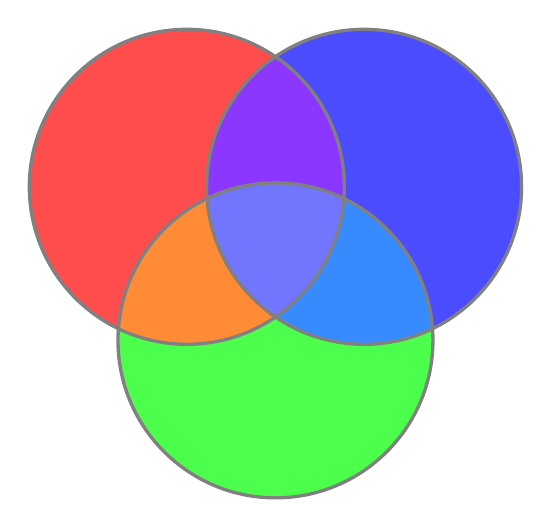
\begin{tikzpicture}
  \begin{scope}[blend group=soft light]
   \fill[blue!70!white] (30:1.3) circle (2cm);
   \fill[red!70!white] (150:1.3) circle (2cm);
   \fill[green!70!white] (270:1.3) circle (2cm);
  \end{scope}
  \draw[gray,very thick] (30:1.3) circle (2cm);
  \draw[gray,very thick] (150:1.3) circle (2cm);
  \draw[gray,very thick] (270:1.3) circle (2cm);
 \end{tikzpicture}
 \caption{Množiny $\clr{A}, \clb{B}, \clg{C}$ s neprázdným průnikem.}
 \label{fig:inkluze-exkluze-1}
\end{figure}

Budeme nyní počítat velikost sjednocení $\clr{A} \cup \clb{B} \cup \clg{C}$.

Za předpokladu, že by množiny byly disjunktní, stačilo by zkrátka sečíst
velikosti jednotlivých množin. V této situaci však započteme některé prvky
vícekrát. Stane se to proto, že když sečtu třeba $\# \clr{A} + \# \clb{B}$, tak
prvky, které leží i v $\clr{A}$ i v $\clb{B}$ (tedy ty v průniku
\textcolor[HTML]{7f33e8}{$A \cap B$}) započtu dvakrát. Na
\hyperref[fig:inkluze-exkluze-2]{obrázku níže} vidíte, kolikrát započteme který
\uv{díl} svého Vennova diagramu.

\begin{figure}[h]
 \centering
 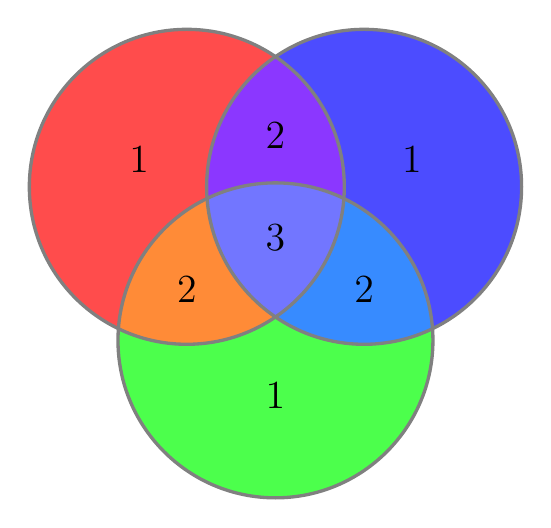
\begin{tikzpicture}
  \begin{scope}[blend group=soft light]
   \fill[blue!70!white] (30:1.3) circle (2cm);
   \fill[red!70!white] (150:1.3) circle (2cm);
   \fill[green!70!white] (270:1.3) circle (2cm);
  \end{scope}
  \draw[gray,very thick] (30:1.3) circle (2cm);
  \draw[gray,very thick] (150:1.3) circle (2cm);
  \draw[gray,very thick] (270:1.3) circle (2cm);
  
  \foreach \angle in {30,150,270} {
   \node at (\angle:2) {\Large $1$};
  }
  \foreach \angle in {90,210,330} {
   \node at (\angle:1.3) {\Large $2$};
  }
  \node at (0,0) {\Large $3$};
 \end{tikzpicture}
 \caption{Znázornění součtu $\# \clr{A} + \# \clb{B} + \# \clg{C}$.}
 \label{fig:inkluze-exkluze-2}
\end{figure}

Jak můžete vyčíst z \hyperref[fig:inkluze-exkluze-2]{obrázku}, některé průniky
jsme započítali mockrát. Černá čísla značí, kolikrát jsme každý kousek
sjednocení započetli, když jsme sečetli $\# \clr{A} + \# \clb{B} + \# \clg{C}$.
Například jsme tedy započetli každý prvek ležící v průniku
$\textcolor[HTML]{e78033}{A \cap C}$ dvakrát a každý prvek v průniku
$\textcolor[HTML]{6a6ee9}{A \cap B \cap C}$ dokonce třikrát.

Abychom situaci napravili, a započetli průnik každého páru množin jen jednou,
odečteme od součtu $\# \clr{A} + \# \clb{B} + \# \clg{C}$ velikosti všech
průniků dvou množin. Odpovídající diagram vidíte
\hyperref[fig:inkluze-exkluze-3]{níže}.

\begin{figure}[h]
 \centering
 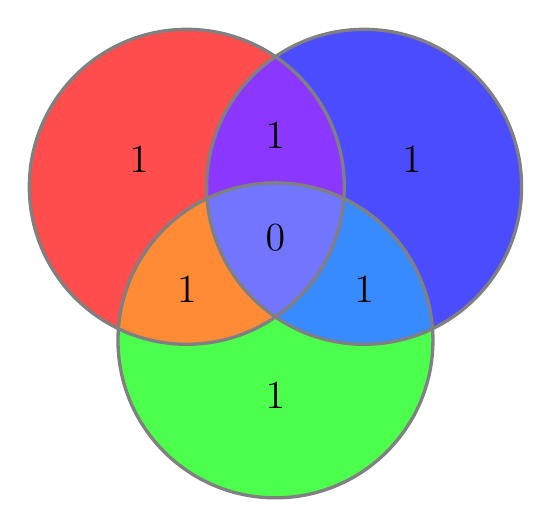
\begin{tikzpicture}
  \begin{scope}[blend group=soft light]
   \fill[blue!70!white] (30:1.3) circle (2cm);
   \fill[red!70!white] (150:1.3) circle (2cm);
   \fill[green!70!white] (270:1.3) circle (2cm);
  \end{scope}
  \draw[gray,very thick] (30:1.3) circle (2cm);
  \draw[gray,very thick] (150:1.3) circle (2cm);
  \draw[gray,very thick] (270:1.3) circle (2cm);
  
  \foreach \angle in {30,150,270} {
   \node at (\angle:2) {\Large $1$};
  }
  \foreach \angle in {90,210,330} {
   \node at (\angle:1.3) {\Large $1$};
  }
  \node at (0,0) {\Large $0$};
 \end{tikzpicture}
 \caption{Znázornění výrazu $\# \clr{A} + \# \clb{B} + \# \clg{C} - \#
 \textcolor[HTML]{7f33e8}{A \cap B} - \# \textcolor[HTML]{e78033}{A \cap C} - \#
 \textcolor[HTML]{3a87ef}{B \cap C}$.}
 \label{fig:inkluze-exkluze-3}
\end{figure}

Ovšem, nyní jsme zase odečetli třikrát průnik $\textcolor[HTML]{6a6ee9}{A \cap B
\cap C}$, protože každý prvek v $\textcolor[HTML]{6a6ee9}{A \cap B \cap C}$ leží
zároveň v $\textcolor[HTML]{7f33e8}{A \cap B}$, v $\textcolor[HTML]{e78033}{A
\cap C}$ i v $\textcolor[HTML]{3a87ef}{B \cap C}$, a ty jsme všechny odečetli.
Tedy nám z průniku $\textcolor[HTML]{6a6ee9}{A \cap B \cap C}$ žádné prvky
nezůstaly. Situaci napravíme tím, že jeho velikost přičteme zpátky. Celkově
dostaneme pro velikost sjednocení $\# A \cup B \cup C$ vzorec
\[
 \# A \cup B \cup C = \# \clr{A} + \# \clb{B} + \# \clg{C} - \#
 \textcolor[HTML]{7f33e8}{A \cap B} - \# \textcolor[HTML]{e78033}{A \cap C} - \#
 \textcolor[HTML]{3a87ef}{B \cap C} + \# \textcolor[HTML]{6a6ee9}{A \cap B \cap
 C}.
\]
Finální znázornění vidíte na
\hyperref[fig:inkluze-exkluze-4]{obrázku~\ref*{fig:inkluze-exkluze-4}}.

\begin{figure}[h]
 \centering
 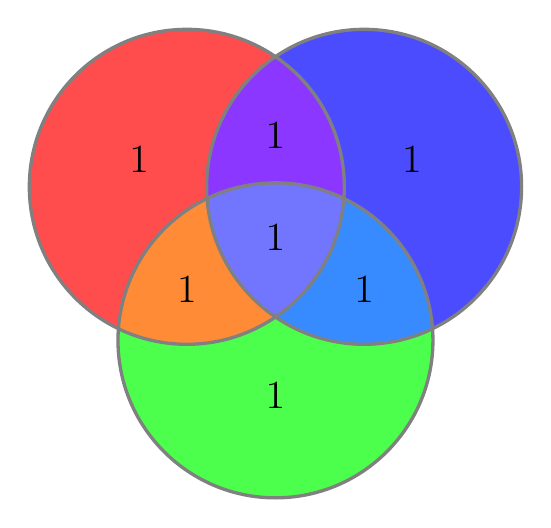
\begin{tikzpicture}
  \begin{scope}[blend group=soft light]
   \fill[blue!70!white] (30:1.3) circle (2cm);
   \fill[red!70!white] (150:1.3) circle (2cm);
   \fill[green!70!white] (270:1.3) circle (2cm);
  \end{scope}
  \draw[gray,very thick] (30:1.3) circle (2cm);
  \draw[gray,very thick] (150:1.3) circle (2cm);
  \draw[gray,very thick] (270:1.3) circle (2cm);
  
  \foreach \angle in {30,150,270} {
   \node at (\angle:2) {\Large $1$};
  }
  \foreach \angle in {90,210,330} {
   \node at (\angle:1.3) {\Large $1$};
  }
  \node at (0,0) {\Large $1$};
 \end{tikzpicture}
 \caption{Velikost sjednocení $\# A \cup B \cup C$ podle principu inkluze a
 exkluze.}
 \label{fig:inkluze-exkluze-4}
\end{figure}

Formální znění principu inkluze a exkluze dí, že tento postup funguje zcela
obecně, tedy že pokud průniky sudého počtu množin odečítám a lichého počtu
přičítám, dostanu tím velikost sjednocení.

Ještě předtím, než ho uvedeme a dokážeme, si ale určíme počet studentů
z~\hyperref[exam:inkluze-exkluze]{úvodního příkladu}. Množiny němčinářů,
španělštinářů a francouzštinářů označíme po řadě $N$, $\check{S}$ a $\check{Z}$
(jako \textbf{ž}abožrout). Ze zadání víme, že $\# N = 30, \# \check{S} = 25$ a
$\# \check{Z} = 2$. Dále víme, že $\# N \cap \check{S} = 4$, protože mezi
němčináři jsou čtyři španělštináři; podobně $\# N \cap \check{Z} = 1$ a $\#
\check{S} \cap \check{Z} = 0$. Konečně, $\# N  \cap \check{S} \cap \check{Z} =
1$. Podle principu inkluze a exkluze máme
\begin{align*}
 \# N \cup \check{S} \cup \check{Z} &= \# N + \# \check{S} + \# \check{Z} - \# N
  \cap \check{S} - \# N  \cap \check{Z} - \# \check{S} \cap \check{Z} + \# N
  \cap \check{S}  \cap \check{Z}\\
 &= 30 + 25 + 2 - 4 - 1 - 0 + 1 = 53.
\end{align*}
Celkem se tedy na Gymnáziu Growth Severní Obec učí 53 studentů cizím jazykům.

Posledním krokem, který zbývá, je umět princip inkluze a exkluze nějak rozumně
zapsat. Tohle je asi první situace, na kterou jsme narazili, kdy bez rozumného
zápisu daného tvrzení bychom se ze symbolů doslova zbláznili (hlavně v jeho
důkazu). Natvrdo napsaný říká princip inkluze a exkluze, že
\begin{align*}
 \# \bigcup_{i=1}^{n} A_i &= \# A_1 + \# A_2 + \cdots + \# A_n\\
 &- \# A_1 \cap A_2 - \# A_1 \cap A_3 - \cdots - \# A_1 \cap A_n - \# A_2
 \cap A_3 - \cdots - \# A_{n-1} \cap A_n\\
 &+ \# A_1 \cap A_2 \cap A_3 + \cdots + \# A_{n-2} \cap A_{n-1} \cap A_n +
 \cdots + (-1)^{n-1} \bigcap_{i=1}^{n} A_i.
\end{align*}
Jak sami vidíte, z tohoto zápisu je sotva (pokud vůbec) poznat, čemu se vlastně
velikost sjednocení $\bigcup_{i=1}^{n} A_i$ rovná. Musíme tento zápis
zjednodušit. Nejprve, pro každou $I \subseteq \{1,\ldots,n\}$ znamená zápis
\[
 \bigcap_{i \in I}^{} A_i
\]
průnik přesně těch množin $A_i$, jejichž indexy leží v množině $I$. Je-li tedy
např. $I = \{1,4,5\}$, pak
\[
 \bigcap_{i  \in I}^{} A_i = A_1 \cap A_4 \cap A_5.
\]
Pro extrémní případ $I = \emptyset$ dodefinujeme $\bigcap_{i \in  I}^{}A_i
\coloneqq \emptyset$, tedy prázdný průnik je prázdná množina.

Dále si rozmyslíme jednoduchý způsob, jak zapsat znaménko u každého z průniků.
Víme, že průnik sudého počtu množin má záporné znaménko a průnik lichého počtu
má kladné. Ještě jinak, když $\# I$ je sudé číslo, pak $\bigcap_{i \in  I}^{}
A_i$ musí dostat záporné znaménko, a když $\# I$ je liché číslo, tak kladné. V
matematice se pro tyto účely obvykle používá $(-1)^{k}$ pro přirozené číslo $k
\in \N$, protože $(-1)^{k}=1$, když $k$ je sudé, a $(-1)^{k} = -1$, když $k$ je
liché. To ale znamená, že výraz $\# \bigcap_{i \in  I}^{} A_i$ musí být
vynásobený číslem $(-1)^{\# I-1}$.

Už jsme skoro hotovi. Pro vyjádření $\# \bigcup_{i=1}^{n} A_i$ pomocí průniků
musíme sečíst velikosti všech průniků $k$ různých množin pro $k$ od $1$ až do
$n$ se správným znaménkem. Čili, musíme sčítat všechny výrazy $(-1)^{\# I - 1}\#
\bigcap_{i \in  I}^{} A_i$ pro všechny podmnožiny $I \subseteq \{1,\ldots,n\}$.

Předchozí diskuse nám umožňuje zapsat princip inkluze a exkluze jako rovnost
\[
 \# \bigcup_{i=1}^{n} A_i = \sum_{I \subseteq \{1,\ldots,n\}}^{} (-1)^{\# I - 1}
 \# \bigcap_{i \in  I}^{} A_i,
\]
kde symbol $\sum_{I \subseteq \{1,\ldots,n\}}^{}$ značí součet přes všechny
\textbf{podmnožiny} množiny $\{1,\ldots,n\}$.

Ještě jednou tedy princip inkluze a exkluze formulujeme jako větu.

\begin{theorem}[Princip inkluze a exkluze]
 \label{thm:princip-inkluze-a-exkluze}
 Ať $A_1,A_2,\ldots,A_n$ jsou množiny. Pak platí rovnost
 \begin{equation*}
  \label{eq:inkluze-exkluze}
  \tag{$\triangle$}
  \# \bigcup_{i=1}^{n} A_i = \sum_{I \subseteq \{1,\ldots,n\}}^{} (-1)^{\# I -
  1} \# \bigcap_{i \in  I}^{} A_i.
 \end{equation*}
\end{theorem}
\begin{proof}
 Důkaz povedeme indukcí podle $n$.

 Když $n = 1$, pak na levé straně rovnosti \eqref{eq:inkluze-exkluze} máme
 \[
  \# \bigcup_{i=1}^{1} A_i = \# A_1
 \]
 a na pravé straně
 \begin{align*}
  \sum_{I \subseteq \{1\}}^{} (-1)^{\# I - 1} \# \bigcap_{i \in  I}^{} A_i &=
  (-1)^{\#\emptyset-1} \# \bigcap_{i  \in \emptyset}^{} A_i + (-1)^{\#\{1\}-1}
  \# \bigcap_{i  \in \{1\}}^{} A_i\\
  &= (-1)^{-1} \cdot 0 + (-1)^{0} \cdot \# A_1 = \# A_1,
 \end{align*}
 protože jediné podmnožiny $\{1\}$ jsou $\emptyset$ a $\{1\}$. Čili pro $n = 1$ 
 rovnost \eqref{eq:inkluze-exkluze} platí.

 Předpokládejme nyní, že rovnost platí pro všechna čísla menší než $n$ a
 dokazujme rovnost pro $n$. Sjednocení na levé straně \eqref{eq:inkluze-exkluze}
 můžeme napsat jako
 \[
  \bigcup_{i=1}^{n} A_i = \clr{\bigcup_{i=1}^{n-1} A_i} \cup \clb{A_n}.
 \]
 Označíme si $\clr{B_1} \coloneqq \clr{\bigcup_{i=1}^{n-1} A_i}$ a $\clb{B_2}
 \coloneqq \clb{A_n}$. Podle principu inkluze a exkluze pro 2 množiny (ten
 můžeme použít z indukčního předpokladu) máme
 \[
  \# \clr{B_1} \cup \clb{B_2} = \# \clr{B_1} + \# \clb{B_2} - \# \clr{B_1} \cap
  \clb{B_2}.
 \]
 Přepsání zpět do množin $A_i$ nám dá
 \[
  \# \bigcup_{i=1}^{n} A_i= \# \clr{\bigcup_{i=1}^{n-1} A_i} \cup \clb{A_n} = \#
  \clr{\bigcup_{i=1}^{n-1} A_i} + \# \clb{A_n} - \#
  \left(\clr{\bigcup_{i=1}^{n-1} A_i} \cap \clb{A_n}\right).
 \]
 Nejprve si uvědomíme, že
 \[
  \left(\clr{\bigcup_{i=1}^{n-1} A_i}\right) \cap \clb{A_n} =
  \bigcup_{i=1}^{n-1} (\clr{A_i} \cap \clb{A_n}),
 \]
 tedy, že je to samé sjednotit množiny $\clr{A_i}$ a pak je proniknout s
 množinou $\clb{A_n}$ jako nejprve proniknout každou množinu $\clr{A_i}$ s
 množinou $\clb{A_n}$ a pak všechny ty průniky sjednotit.

 Teď můžeme (opět z indukčního předpokladu) použít princip inkluze a exkluze na
 sjednocení $\bigcup_{i=1}^{n-1} \clr{A_i}$ a zároveň na $\bigcup_{i=1}^{n-1}
 (\clr{A_i} \cap \clb{A_n})$.

 Dostaneme
 \[
  \# \bigcup_{i=1}^{n-1} \clr{A_i} = \sum_{I \subseteq \{1,\ldots,n-1\}}
  (-1)^{\# I - 1} \# \bigcap_{i \in  I}^{} \clr{A_i}
 \]
 a
 \[
  \# \bigcup_{i=1}^{n-1} (\clr{A_i} \cap \clb{A_n}) = \sum_{I \subseteq
  \{1,\ldots,n-1\}}^{} (-1)^{\# I - 1} \# \bigcap_{i \in  I}^{} (\clr{A_i} \cap
  \clb{A_n}). 
 \]
 Na jedné straně tedy máme vyjádření
 \begin{equation}
  \label{eq:ink-exk-1}
  \begin{split}
   \# \bigcup_{i=1}^{n} A_i &= \sum_{I \subseteq \{1,\ldots,n-1\}}^{} (-1)^{\# I -
   1} \# \bigcap_{i \in  I}^{} \clr{A_i} + \# \clb{A_n}\\
   &- \sum_{I \subseteq \{1,\ldots,n-1\}}^{} (-1)^{\# I - 1} \# \bigcap_{i \in
   I}^{} (\clr{A_i} \cap \clb{A_n}).
  \end{split}
 \end{equation}
 Na druhé straně potřebujeme dokázat (\textbf{ještě to nevíme!}), že
 \begin{equation}
  \label{eq:ink-exk-2}
  \# \bigcup_{i=1}^{n} A_i  \overset{?}{=} \sum_{I \subseteq \{1,\ldots,n\}}^{}
  (-1)^{\# I - 1} \# \bigcap_{i \in  I}^{} A_i.
 \end{equation}
 Porovnáváme tedy součty na pravých stranách rovností \eqref{eq:ink-exk-1} a
 \eqref{eq:ink-exk-2}. Jediný rozumný způsob, jak to udělat, je podívat se, že
 každý sčítanec v~\eqref{eq:ink-exk-2} je rovněž sčítancem v
 \eqref{eq:ink-exk-1}.

 Rozlišíme dva případy podle toho, zda podmnožina $I$ obsahuje $n$, či ne.
 \begin{enumerate}[label=(\alph*)]
  \item Ať nejprve $n \notin I$. Pak v sumě \eqref{eq:ink-exk-2} je sčítanec
   \[
    (-1)^{\# I-1} \# \bigcap_{i \in  I}^{} A_i,
   \]
   kde ten průnik neobsahuje $A_n$, protože $n \notin I$. Jenže pak je $I
   \subseteq \{1,\ldots,n-1\}$, a tedy i součet \eqref{eq:ink-exk-1} obsahuje
   ten samý sčítanec (v té úplně první sumě nahoře) se stejným znaménkem.
  \item Teď předpokládáme, že $n \in I$. Musíme rozlišit zase dva případy (xD).
   \begin{enumerate}[label=(\greek*)]
    \item $I = \{n\}$. Pak součet \eqref{eq:ink-exk-2} obsahuje sčítanec
     \[
      (-1)^{\#\{n\}-1} \# \bigcap_{i \in \{n\}}^{} A_i = \# A_n,
     \]
     který je ale i v součtu \eqref{eq:ink-exk-1} (mezi těmi dvěma sumami).
    \item $I$ obsahuje $n$ a $\# I \geq 2$. V tomto případě máme v součtu
     \eqref{eq:ink-exk-2} sčítanec
     \[
      (-1)^{\# I - 1} \# \bigcap_{i \in I}^{} A_i,
     \]
     jejž si však můžeme přepsat jako
     \begin{align*}
      (-1)^{\# I - 1} \# \bigcap_{i \in I}^{} A_i &= (-1)^{\# I - 1} \#
      \left(\bigcap_{i \in  I \setminus \{n\}}^{} \clr{A_i}\right) \cap
      \clb{A_n}\\
      &= (-1)^{\# I - 1} \# \bigcap_{i  \in I \setminus \{n\}}^{} (\clr{A_i}
      \cap \clb{A_n}),
     \end{align*}
     jelikož předpokládáme, že $n \in I$. Protože $I \setminus \{n\} \subseteq
     \{1,\ldots,n-1\}$, je v součtu \eqref{eq:ink-exk-1} (v té sumě dole)
     sčítanec
     \[
     (-1)^{\#(I \setminus \{n\}) - 1} \# \bigcap_{i  \in I \setminus \{n\}}^{}
     (\clr{A_i} \cap \clb{A_n}),
     \]
     což je v podstatě tentýž, až na znaménko. To však není problém, neboť si
     můžete všimnout, že v součtu \eqref{eq:ink-exk-1} tu druhou sumu obsahující
     všechny průniky s množinou $\clb{A_n}$ odečítám. Tedy, odpovídající
     sčítanec má ve skutečnosti znaménko $-(-1)^{\# (I \setminus \{n\})-1} =
     (-1)^{\# I - 1}$.
   \end{enumerate}
 \end{enumerate}
 Tím jsme ověřili, že součet ve vyjádření \eqref{eq:ink-exk-1} obsahuje přesně
 tytéž sčítance jako součet ve vyjádření \eqref{eq:ink-exk-2}, a tudíž se jedná
 o stejný součet. Tím je podle principu matematické indukce důkaz dokončen.
\end{proof}

Nakonec se podíváme, že
\hyperref[thm:princip-inkluze-a-exkluze]{věta~\ref*{thm:princip-inkluze-a-exkluze}}
souhlasí plně s naší intuicí v již prozkoumaném případě tří množin s neprázdným
průnikem.

\begin{example}
 Uvažme množiny $A_1,A_2,A_3$ takové, že $A_1 \cap A_2 \cap A_3 \neq \emptyset$.
 Podle \hyperref[thm:princip-inkluze-a-exkluze]{principu inkluze a exkluze}
 počítáme
 \[
  \# A_1 \cup A_2 \cup A_3 = \sum_{I \subseteq \{1,2,3\}}^{} (-1)^{\#I - 1}\#
  \bigcap_{i \in  I}^{} A_i.
 \]
 Jednoprvkové podmnožiny $\{1,2,3\}$ jsou $\{1\}, \{2\}$ a $\{3\}$. Tedy
 započteme
 \[
  (-1)^{1-1} \# A_1 + (-1)^{1-1}\# A_2 + (-1)^{1-1}\# A_3 = \# A_1 + \# A_2 + \#
  A_3.
 \]
 Ty dvouprvkové jsou $\{1,2\}, \{1,3\}$ a $\{2,3\}$. Dávají nám po řadě sčítance
 \begin{align*}
  &(-1)^{2-1}\# A_1 \cap A_2 + (-1)^{2-1}\# A_1 \cap A_3 + (-1)^{2-1}\# A_2 \cap
  A_3\\
  &= -\# A_1 \cap A_2 - \# A_1 \cap A_3 - \#A_2 \cap A_3.
 \end{align*}
 Konečně, tříprvkovou podmnožinu má $\{1,2,3\}$ jenom jednu -- sebe samu. Za tu
 si započteme
 \[
  (-1)^{3-1}\#A_1 \cap A_2 \cap A_3 = \# A_1 \cap A_2 \cap A_3.
 \]
 Když sečteme průniky přes všechny podmnožiny $\{1,2,3\}$, dostaneme
 \begin{align*}
  \# A_1 \cup A_2 \cup A_3 &= \#A_1 + \#A_2 + \#A_3\\
  &-\#A_1 \cap A_2 - \#A_1 \cap A_3 - \#A_2 \cap A_3\\
  &+ \# A_1 \cap A_2 \cap A_3,
 \end{align*}
 jak jsme očekávali.
\end{example}

Kterak káže obyčej, pár cvičení závěrem.

\begin{exercise}[zase trocha teorie čísel]
 Jeden z oblíbených a celkem rychlých rozkladů čísla na prvočísla je tzv.
 \emph{Eratosthenovo síto}.
 
 Funguje na principu vyškrtávání násobků čísel. Konkrétně, algoritmus prochází
 seznam čísel až do nějaké hranice, a kdykoli narazí na ještě neodškrtnuté
 číslo, odškrtne z tohoto seznamu všechny jeho násobky kromě něho samotného.
 Sami si rozmyslete, že tímto způsobem zůstanou ve výsledném seznamu pouze
 prvočísla.

 My si tady rozmyslíme pouze zjednodušenou verzi. Spočtěte, kolik zůstane čísel
 mezi $1$ a $1000$ potom, co vyškrtáme všechny násobky čísel $2,3,5$ a $7$.
\end{exercise}

\begin{exercise}
 Určete počet přirozených čísel menších než $100$, které nedělí druhá mocnina
 žádného přirozeného čísla (kromě $1$).
\end{exercise}

\begin{exercise}
 Kolika způsoby lze seřadit do řady 5 Čechů, 4 Maďary a 3 Rusy, aby všichni
 příslušníci jednoho národa nikdy nestáli hned za sebou?
\end{exercise}

\subsubsection{Problém šatnářky}
\label{sssec:problem-satnarky}

Kapitolu o kombinatorickém počítání završíme klasickým \emph{problémem
šatnářky}. Jeho tradiční znění je následující.

V jeden chladný podvečer přijde skupina pánů do luxusního podniku. Před vstupem
do lokálu si každý z nich odloží svoji černou buřinku (neb jiné se nenosí) v
pánské šatně. Večírek se však neobyčejně prodlužuje a šatnářka, navíc ten den
dosti nevyspalá, počne únavou podřimovati. Když ctihodní pánové konečně
doflámují, sotva bdělá šatnářka jim při odchodu z šatny náhodně rozdá -- jejíma
zaslepenýma očima nerozlišitelné -- černé buřinky. S jakou pravděpodobností
odchází každý pán s cizí buřinkou?

Očíslujeme si pány přirozenými čísly od $1$ do $n$ a jejich buřinky taktéž; čili
pánovi číslo $i$ připadá buřinka číslo $i$. Náhodné rozdání buřinek odpovídá
výběru permutace $\sigma \in S_n$, neboli bijektivního zobrazení  $\sigma:
\{1,\ldots,n\} \to \{1,\ldots,n\}$. Podle \cref{prop:pocet-permutaci-na-mnozine}
je počet těchto roven $n!$. Jednu konkrétní volbu rozloučení buřinek učiní tedy
šatnářka ze zadání problému s pravděpodobností $1 / n!$. Označíme-li si počet
permutací, které žádné číslo nezobrazují na totéž, jako  $\check{s}(n)$, pak
řešením problému šatnářky je číslo $\check{s}(n) / n!$.

Tou netriviální otázkou zůstává, jak $\check{s}(n)$ určit. Postup, který se zde
jmeme popsat, využívá \uv{trik} častý především v teorii pravděpodobnosti. Bývá
totiž obvykle výrazně jednodušší spočítat počet objektů, které \textbf{splňují}
nějakou vlastnost, raději než objektů, které onu vlastnost \textbf{nesplňují}.
Oba postupy jsou logicky ekvivalentní, neboť počet objektů nesplňujících
vlastnost $V$ je roven rozdílu počtu všech objektů a počtu těch, které vlastnost
$V$ splňují. Výpočetně se však postupy svou obtížností často výrazně liší.

Místo toho, abychom určovali počet permutací $\sigma \in S_n$, jež nezobrazí
žádný prvek na sebe, budeme počítat permutace, které zobrazí aspoň jeden prvek
na sebe. Takovému prvku se pak obvykle říká \emph{pevný bod} dané permutace.

\begin{definition}[Pevný bod]
 \label{def:pevny-bod}
 Ať $\sigma \in S_n$. Prvek $i  \in \{1,\ldots,n\}$ nazveme \emph{pevným bodem}
 permutace $\sigma$, pokud $\sigma(i) = i$.
\end{definition}

Pro dané $i  \in \{1,\ldots,n\}$ si ještě označíme
\[
 \mathcal{P}_i \coloneqq \{\sigma \in S_n \mid \sigma(i) = i\},
\]
čili $\mathcal{P}_i$ je množina permutací, jejichž pevným bodem (\textbf{možná
ne jediným!}) je $i$. Snadno si rozmyslíme, že množina všech permutací, které
mají \textbf{aspoň jeden pevný bod}, je právě
\[
 \mathcal{P}_1 \cup \mathcal{P}_2  \cup \ldots \cup \mathcal{P}_n =
 \bigcup_{i=1}^{n} \mathcal{P}_i.
\]
Vskutku, permutace $\sigma$ leží v $\bigcup_{i=1}^{n} \mathcal{P}_i$ právě
tehdy, když existuje nějaké ${i  \in \{1,\ldots,n\}}$ takové, že $\sigma(i) =
i$, což je z \hyperref[def:pevny-bod]{definice} právě tehdy, když existuje
nějaký její pevný bod. Čili, $\# \bigcup_{i=1}^{n} \mathcal{P}_i$ vyjadřuje
počet permutací, které zobrazí aspoň jeden prvek na ten samý. Z diskuse výše
plyne, že
\[
 \check{s}(n) = n! - \# \bigcup_{i=1}^{n} \mathcal{P}_i.
\]
Problém šatnářky vyřešíme tím, že určíme $\# \bigcup_{i=1}^{n} \mathcal{P}_i$. Z
\myref{věty}{thm:princip-inkluze-a-exkluze} můžeme počítat
\begin{equation*}
 \label{eq:aspon-jeden-pevny-bod}
 \tag{$\square$}
 \# \bigcup_{i=1}^{n} \mathcal{P}_i = \sum_{I \subseteq \{1,\ldots,n\}}^{}
 (-1)^{\# I-1}\# \bigcap_{i \in  I}^{} \mathcal{P}_i.
\end{equation*}
Dalším krokem ke zdárnému řešení problému je uvědomění, že výraz $\# \bigcap_{i
\in  I}^{} \mathcal{P}_i$ záleží pouze na $\# I$, nikoli na konkrétních
indexech, které se v~$I$ vyskytují. Přeci, $\# \bigcap_{i \in  I}^{}
\mathcal{P}_i$ značí počet permutací s přesně $\# I$ pevnými body. Všimněme si,
že ten je určen pouze samotným počtem pevných bodů, a ne jejich konkrétní
hodnotou.

Toto pozorování napovídá, že v součtu na pravé straně
\eqref{eq:aspon-jeden-pevny-bod} můžeme sloučit ty sčítance, pro něž je $\# I$
stabilní. Řečeno přímočařeji, stačí, když budeme sčítat pouze přes
\textbf{velikosti} všech podmnožin, a nemusíme sčítat přes individuální
podmnožiny, neboť na jejich konkrétních prvcích nezáleží (pouze na jejich
velikostech).

Provedeme pro přehlednost ještě poslední přeznačení. Výraz $\mathsf{P}(k)$ bude
značit \emph{počet} permutací s přesně $k$ pevnými body. Díky předchozímu
odstavci bychom též mohli být formální a psát, že
\[
 \mathsf{P}(k) = \sum_{\substack{I \subseteq \{1,\ldots,n\}\\ \#I = k}}
 \#\bigcap_{i \in  I}^{} \mathcal{P}_i,
\]
čili (dokonce správně) tvrdit, že počet permutací s $k$ pevnými body dostaneme
tak, že sečteme počty permutací s pevnými body v podmnožině $I$ přes všechny
$k$-prvkové podmnožiny $I$.

Nyní můžeme rovnost \eqref{eq:aspon-jeden-pevny-bod} přepsat do mnohem
jednodušší podoby
\[
 \# \bigcup_{i=1}^{n} \mathcal{P}_i = \sum_{k=1}^{n} (-1)^{k-1} \mathsf{P}(k).
\]
Opět přeloženo do lidské řeči říkáme, že počet permutací s aspoň jedním pevným
bodem můžeme určit jako součet (až na znaménko) všech permutací s přesně $k$
pevnými body přes všechna $k$ od $1$ do $n$. To dává smysl.

Dokážeme-li určit $\mathsf{P}(k)$, jsme hotovi. K tomu slouží následující lemma.

\begin{lemma}
 \label{lemma:permutace-s-k-pevnymi-body}
 Ať $k \in\N, k \leq n$. Platí
 \begin{equation*}
  \label{eq:k-pevnych-bodu}
  \tag{$\bullet$}
  \mathsf{P}(k) = \binom{n}{k}(n-k)! = \frac{n!}{k!}.
 \end{equation*}
\end{lemma}
\begin{proof}
 Za důkaz vřele děkujeme laureátovi Fieldsovy medaile, prof. Mgr. et Ing.
 Jáchymovi Löwenhöfferu, RNDr. et Ph. D., CSc., DSc. Neodvažujeme se však přímo
 parafrázovat, tedy jej s odpuštěním mírně přeformulujeme.

 Permutace s přesně $k$ libovolnými pevnými body je určena výběrem těchto $k$ 
 pevných bodů z $n$ čísel a poté výběrem uspořádání zbývajících $n-k$ čísel.
 Výběr $k$ prvků z $n$ mohu podle
 \myref{tvrzení}{claim:pocet-k-prvkovych-podmnozin} učinit $\binom{n}{k}$
 způsoby. Zvolit permutaci zbývajících $n-k$ prvků mohu podle
 \myref{tvrzení}{prop:pocet-permutaci-na-mnozine} $(n-k)!$ způsoby. Celkem tedy
 mohu určit jednu permutaci na $n$ prvcích s $k$ pevnými body přesně
 $\binom{n}{k}(n-k)!$ způsoby. To dokazuje první rovnost v
 \eqref{eq:k-pevnych-bodu}.

 Ta druhá plyne z \myref{lemmatu}{lem:vzorec-pro-kombinacni-cislo}, neboť
 \[
  \binom{n}{k}(n-k)! = \frac{n!}{k!(n-k)!}(n-k)! = \frac{n!}{k!}.\qedhere
 \]
\end{proof}

Dopracovali jsme se k závěru problému. Díky
\hyperref[lemma:permutace-s-k-pevnymi-body]{předchozímu lemmatu} máme po
dosazení do \eqref{eq:aspon-jeden-pevny-bod} vzorec
\[
 \# \bigcup_{i=1}^{n} \mathcal{P}_i = \sum_{k=1}^{n} (-1)^{k-1} \frac{n!}{k!}.
\]
Čili,
\[
 \check{s}(n) = n! - \# \bigcup_{i=1}^{n} \mathcal{P}_i = n! - \sum_{k=1}^{n}
 (-1)^{k-1} \frac{n!}{k!}.
\]
Vytknutí čísla $n!$ dá snad hezčí vyjádření
\[
 \check{s}(n) = n! \sum_{k=0}^{n} (-1)^{k} \frac{1}{k!}.
\]
Je triviální dokázat, že součet výše konverguje k $1 / e$, kde písmeno $e$ značí
tzv. \href{https://cs.wikipedia.org/wiki/Eulerovo_%C4%8D%C3%ADslo}{Eulerovo
číslo}. Formálně zapsáno,
\[
 \sum_{k=0}^{n} (-1)^{k} \frac{1}{k!} \xrightarrow{n \to \infty}
 \frac{1}{e}.
\]
Neformálně tento vztah říká, že čím je vyšší počet přišedších pánů do podniku,
tím víc se pravděpodobnost, že šatnářka vrátí každému cizí buřinku, blíží k
číslu $1 / e$. Je tomu tak pro to, že
\[
 \frac{\check{s}(n)}{n!} = \frac{n!\sum_{k=0}^{n} (-1)^{k} \frac{1}{k!}}{n!} =
 \sum_{k=0}^{n} (-1)^{k} \frac{1}{k!} \xrightarrow{n \to \infty} \frac{1}{e},
\]
kde, pamatujte, $\check{s}(n) / n!$ je přesně řešení problému šatnářky.

